\chapter{Voltage Sources and References}
Voltage sources are circuits designed to maintain a constant voltage and supply a load current to other circuitry. Voltage references also maintain a constant voltage for other circuitry (for example, to bias a one input of a comparator so that the comparator's output is high when its input is at a higher voltage than the voltage reference and low otherwise). Unlike voltage sources, however, voltage references are usually not required to supply a significant load current. Ideally, the voltage output $v_{O}$ of voltage references and sources does not vary with the load current and $v_{O}$ has no AC component (it is a pure DC voltage). In practice, higher load currents often cause $v_{O}$ to decrease slightly because the voltage reference/source has a nonzero output resistance $R_{o}$. If the input voltage is $v_{I}$ and the load current $i_{L}$, then the output voltage is

\begin{equation}
v_{O} = v_{I} - i_{L}R_{o}
\end{equation}

\noindent It is crucial, therefore, for a voltage source to have a low $R_{o}$. Voltage references should also have a low $R_{o}$, but they do not need to supply larger load currents so $v_{O} \approx v_{I}$ even if $R_{o}$ is significant. Also in practice, AC noise is present in the output. One way to minimize AC noise is to add a low pass filter after the voltage source/reference to help remove the high frequency noise. However, the low pass filter will affect $R_{o}$.
%http://en.wikipedia.org/wiki/Image:Op-amp_current_source_with_pass_transistor.png
\section{Resistor divider}
\begin{center}
	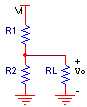
\includegraphics{schematics/resistordivider.PNG}
\end{center}
The resistor divider is the simplest voltage source or reference possible. Its transfer function (unloaded) can be determined by inspection:

\begin{equation}
v_{O} = \frac{R_{2}v_{I}}{R_{1}+R_{2}}
\end{equation}

\noindent When loaded by a resistance $R_{L}$, the transfer function is the same but with $R_{2}$ replaced by $R_{2}||R_{L}$. Specifically,

\textcolor{red}{
\begin{equation}
v_{O} = \frac{R_{2}R_{L}v_{I}}{R_{1}(R_{2}+R_{L})+R_{2}R_{L}}
\end{equation}
}

\noindent The output resistance $R_{o}$ is also easy to determine -- with $v_{I} = 0$ the two resistors are in parallel looking into the output:

\textcolor{red}{
\begin{equation}
R_{o} = \frac{R_{1}R_{2}}{R_{1}+R_{2}}
\end{equation}
}

\noindent $R_{o}$ is usually quite high since $R_{1}$ and $R_{2}$ must be large enough that the current drawn by the circuit is not unnecessarily high. Consequently, the simple resistor divider is a poor voltage source and is often only used as a voltage reference.

\section{Resistor divider with emitter/source follower}
\begin{center}
	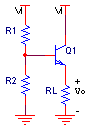
\includegraphics{schematics/resistordivider_emitterfollower.PNG}
\end{center}

One way to improve $R_{o}$ of the resistor divider is to connect an emitter/source follower to the output. An emitter/source follower has a high input resistance so that the load current seen by the resistor divider is low, but it also has a low output resistance. The drawback is that $v_{O}$ is lower by approximately $v_{BE}$ or $v_{GS}$ due to the transistor. More specifically, $v_{O}$ is dependent on the load current $i_{L}$ since

\begin{equation}
v_{O} = i_{L}R_{L}
\end{equation}

For an emitter follower, the relationship between $i_{L}$ and $v_{BE}$ is given by (\ref{eq:bipolarIc}). Since

\begin{equation}
i_{L} = i_{E} = \frac{\beta_{F}+1}{\beta_{F}}i_{C}
\end{equation}

\noindent we can use (\ref{eq:bipolarIc}) to find $v_{BE}$ in terms of $i_{L}$:

\begin{equation}
v_{BE} = V_{th}\ln\left(\frac{\beta_{F}i_{L}}{(\beta_{F}+1)I_{S}}\right)
\end{equation}

\noindent The transfer function is therefore

\textcolor{red}{
\begin{equation}
v_{O} = \frac{R_{2}v_{I}}{R_{1}+R_{2}} - V_{th}\ln\left(\frac{\beta_{F}i_{L}}{(\beta_{F}+1)I_{S}}\right)
\end{equation}
}

The output resistance $R_{o}$ is simply that of an emitter follower, given by (\ref{eq:emitter_follower_Ro}). In terms of the above circuit it is

\textcolor{red}{
\begin{equation}
R_{o} = \frac{(R_{1}||R_{2})+r_{\pi}}{\beta_{F}+1}||r_{o}
\end{equation}
}

If a source follower is used instead then the relationship between $i_{L}$ and $v_{GS}$ is given by (\ref{eq:activeId}). For the MOS transistor

\begin{equation}
i_{L} = i_{D}
\end{equation}

\noindent so we can solve for $v_{GS}$ in (\ref{eq:activeId}) to find $v_{GS}$ in terms of $i_{L}$:

\begin{equation}
v_{GS} = V_{t} + \sqrt{\frac{L}{W}\frac{2I_{D}}{\mu_{n}C_{ox}}\left(1+\frac{V_{DS}}{V_{A}}\right)}
\end{equation}

\noindent The transfer function is therefore

\textcolor{red}{
\begin{equation}
v_{O} = \frac{R_{2}v_{I}}{R_{1}+R_{2}} - \left(V_{t} + \sqrt{\frac{L}{W}\frac{2I_{D}}{\mu_{n}C_{ox}}\left(1+\frac{V_{DS}}{V_{A}}\right)}\right)
\end{equation}
}

\noindent and the output resistance $R_{o}$ is the same as (\ref{eq:sourcefollower_Ro}):

\textcolor{red}{
\begin{equation}
R_{o} = \frac{1}{g_{m}+g_{mb}+\frac{1}{r_{o}}+\frac{1}{R_{L}}}
\end{equation}
}

\section{Resistor divider with operational amplifier buffer}
\begin{center}
	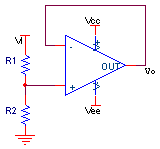
\includegraphics{schematics/resistordivider_opampbuffer.PNG}
\end{center}
The best way to improve the output resistance of $R_{o}$ of the resistor divider is to use an operational amplifier buffer on the output (although the use of a full operational amplifier may be unnecessary or undesirable). Unlike the emitter/source follower, the output voltage is not lowered by a $v_{BE}$ (or $v_{GS}$) drop and is simply

\textcolor{red}{
\begin{equation}
v_{O} = \frac{R_{2}v_{I}}{R_{1}+R_{2}}
\end{equation}
}

\noindent The output resistance $R_{o}$ is simply the operational amplifier's $R_{o}$.

\section{Zener diode regulator}
\begin{center}
	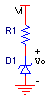
\includegraphics{schematics/zenerdiode_regulator.PNG}
\end{center}

The Zener diode regulator relies on a Zener diode's reverse-bias breakdown voltage -- the reverse-bias voltage $V_{Z}$ at which a Zener diode begins to conduct current. The Zener diode has a low impedance at $V_{Z}$ so the reverse-bias voltage remains mostly constant even over a wide range of reverse current through the diode. The series resistor $R_{1}$ limits the current through the diode. As long as $V_{I} > V_{Z}$ and the current through the diode is nonzero

\textcolor{red}{
\begin{equation}
v_{O} = V_{Z}
\end{equation}
}

\noindent The output resistance $R_{o}$ is approximately the (low) resistance of the Zener diode in reverse breakdown, $R_{Z}$, since generally $R_{1} >> R_{Z}$ and

\textcolor{red}{
\begin{equation}
R_{o} = R_{1}||R_{Z} \approx R_{Z}
\end{equation}
}

As with the resistor divider, the simple Zener diode regulator can be improved by adding an emitter/source follower or operational amplifier buffer to the output. In this case, the emitter/source follower or operational amplifier buffer help ensure that the reverse-bias voltage across the diode remains greater than the diode's reverse-bias breakdown voltage.

\section{$V_{BE}$ multiplier}
\begin{center}
	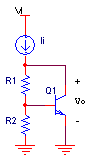
\includegraphics{schematics/vbe_multiplier.PNG}
\end{center}

The $V_{BE}$ multiplier requires a bipolar transistor with a high $\beta_{F}$. If $\beta_{F} >> 1$ then $I_{B}$ (the base current into the transistor) is negligible. With that assumption the current $I$ through $R_{1}$ is equal to the current through $R_{2}$. Since the current through the resistors is nearly equal

\begin{equation}
V_{O} = I(R_{1}+R_{2})
\end{equation}

\noindent The voltage across $R_{2}$ is equal to $V_{BE}$ so

\begin{equation}
I = \frac{V_{BE}}{R_{2}}
\end{equation}

\noindent and thus

\textcolor{red}{
\begin{equation}
V_{O} = V_{BE}\left(1+\frac{R_{1}}{R_{2}}\right)
\label{eq:vbe_multiplier_Vo}
\end{equation}
}

To choose the appropriate $I_{I}$, make sure $Q_{1}$ is in the forward active region (so that $\beta_{F} >> 1$):

\begin{equation}
V_{BE1} > 0
\end{equation}

\noindent and

\begin{equation}
V_{CE1} > V_{CE(\text{sat})}
\end{equation}

\section{Widlar bandgap reference (GHLM p. 323)}
\begin{center}
	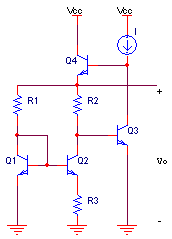
\includegraphics{schematics/Widlar_bandgap.PNG}
\end{center}
The Widlar bandgap reference circuit has two stable operating points but only one desirable operating point, so a start-up circuit (not shown above) is required to ensure that the circuit reaches the desirable operating point. Assuming the circuit is in the desired stable operating point,

\begin{equation}
V_{O} = V_{BE3} + V_{R2}
\label{eq:Widlar_bandgap_Vo_basic}
\end{equation}

\noindent where $V_{R2}$ is the voltage across $R_{2}$. The current through $R_{2}$ is approximately equal to $R_{3}$ if $Q_{2}$'s $\beta_{F} >> 1$, in which case

\begin{equation}
V_{R2} = I_{C2}R_{2} = \frac{R_{2}}{R_{3}}V_{R3}
\label{eq:Widlar_bandgap_Vr2_wrt_Vr3}
\end{equation}

\noindent and the voltage across $R_{3}$ is

\begin{equation}
V_{R3} = V_{BE1} - V_{BE2} = V_{T}\ln\left(\frac{I_{C1}}{I_{C2}}\frac{I_{S2}}{I_{S1}}\right)
\end{equation}

\noindent The ratio of $I_{C1}$ to $I_{C2}$ is determined by the ratio of $R_{2}$ to $R_{1}$, so %TODO: why?????????

\begin{equation}
V_{R3} = V_{T}\ln\left(\frac{R_{2}}{R_{1}}\frac{I_{S2}}{I_{S1}}\right)
\label{eq:Widlar_bandgap_Vr3_R}
\end{equation}

\noindent Substituting (\ref{eq:Widlar_bandgap_Vr3_R}) into (\ref{eq:Widlar_bandgap_Vr2_wrt_Vr3}),

\begin{equation}
V_{R2} = \frac{R_{2}}{R_{3}}V_{T}\ln\left(\frac{R_{2}}{R_{1}}\frac{I_{S2}}{I_{S1}}\right)
\label{eq:Widlar_bandgap_Vr2_R}
\end{equation}

\noindent Substituting (\ref{eq:Widlar_bandgap_Vr2_R}) into (\ref{eq:Widlar_bandgap_Vo_basic}),

\textcolor{red}{
\begin{equation}
V_{O} = V_{BE3} + \frac{R_{2}}{R_{3}}\ln\left(\frac{R_{2}}{R_{1}}\frac{I_{S2}}{I_{S1}}\right)V_{T}
\end{equation}
}

\noindent The base-emitter voltage is inversely proportional to temperature and the voltage across $R_{2}$ is PTAT (proportional to absolute temperature) due to the temperature dependence of $V_{T}$, so an appropriate choice of the multiplicative factor to $V_{T}$ cancels the temperature coefficent for $V_{O}$ at the desired temperature. The multiplicative factor is determined by three ratios: $R_{2}$ to $R_{3}$, $R_{2}$ to $R_{1}$, and $I_{S2}$ to $I_{S1}$.\footnote{Gray, Paul R., et al., "Analysis and Design of Analog Integrated Circuits, Fourth Edition", John Wiley and Sons, Inc., 2001, pp. 322-323}

%\section{Improved Widlar bandgap reference (GHLM p. 323)}

%\section{Brokaw bandgap reference}
%http://en.wikipedia.org/wiki/Brokaw_bandgap_reference

%\section{Op amp voltage regulator (p.230)}